\begin{frame}
%mettre cette slide un peu avant la conclusion
\frametitle{Automata Network modelling of Biological Networks}
\textbf{Transition-centered specification}
\begin{itemize}
\item ...in opposition to function-centered of Boolean/Thomas networks
\item explicit context/ \tval{causality of state changes}
\item closely related to (safe) Petri nets
\item step semantics (purely async, purely sync, mixed)
\end{itemize}
\textbf{Modelling}
\begin{itemize}
\item any Boolean/Thomas networks can be encoded;
\item in case of logical rules uncertainty: \tval{model the union} of Boolean/Thomas networks (over-approximation of behaviours)
%\item encoding of \tval{SBGN Process Description} models
\end{itemize}
\end{frame}

\begin{frame}[c]
 \frametitle{Case study}
 

\tval{Lambda phage} : ($4$  components and $11$  interactions); 

\tval{EGF/TNF} : ($28$  components and $55$  interactions); 

\tval{t\_helper differentiation}: ($101$  components and $381$  interactions).

\begin{center}
  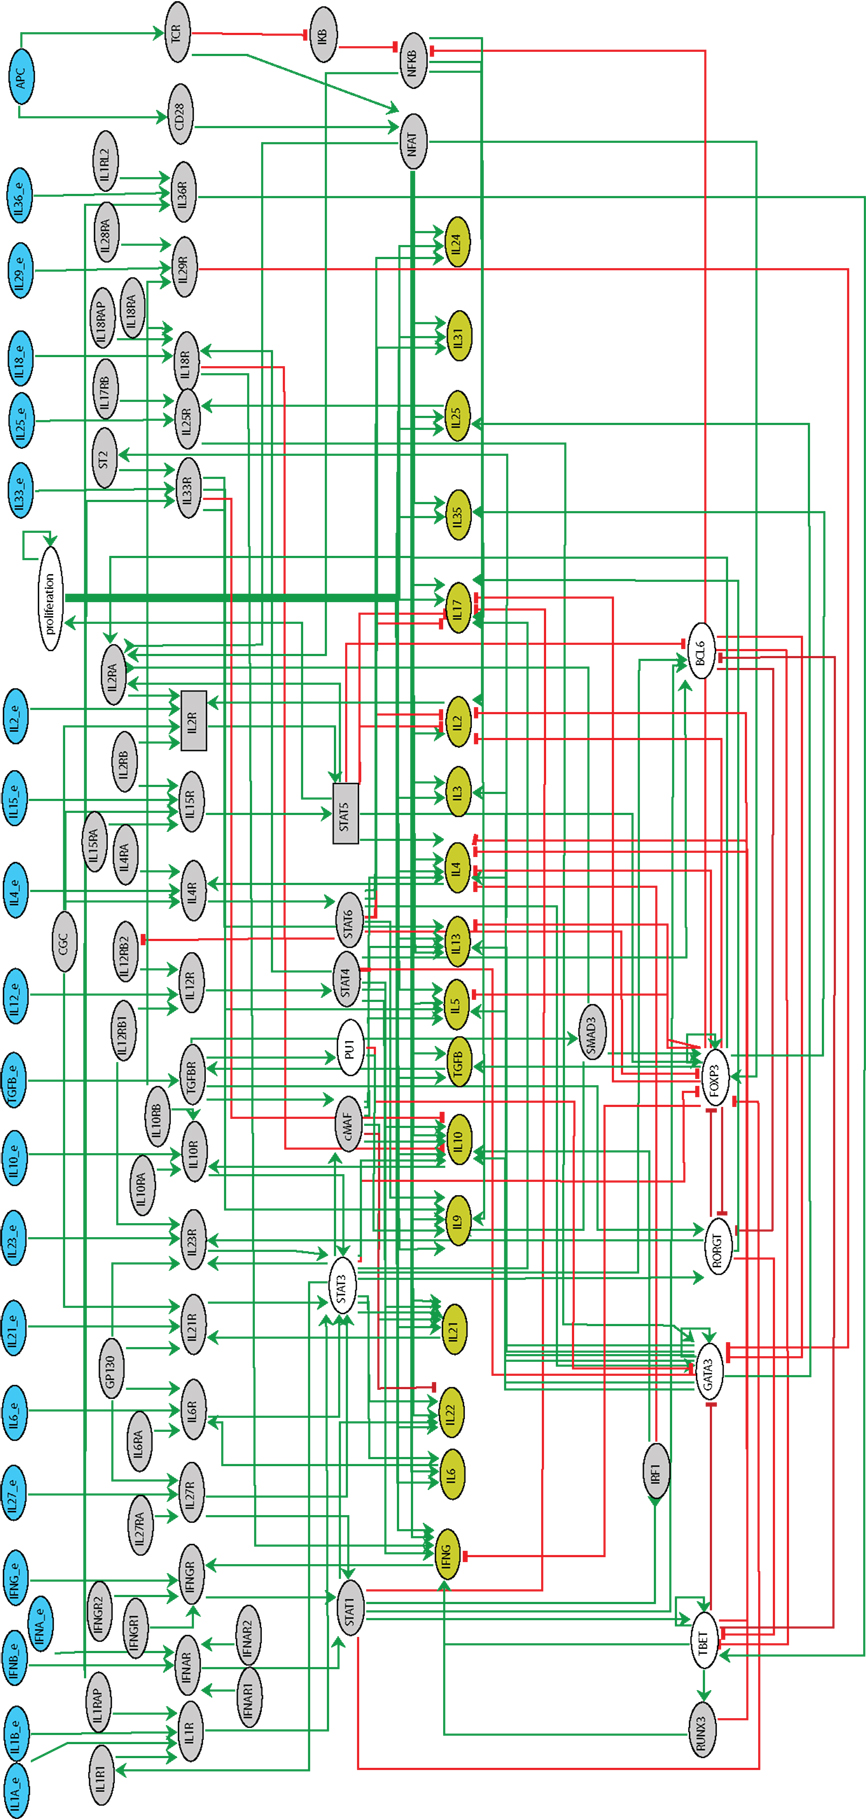
\includegraphics[scale=0.18,angle=-90]{images/th_differentiation.jpg}
\end{center}
\begin{center}
 {\tiny \color{darkgreen} [\citeatfb]}
\end{center}
\end{frame}



%mettre le tableau
\begin{frame}[c]
 \frametitle{Results of identification of bifurcations}
 

%mettre le tableau
\begin{table}[bt]
\renewcommand{\arraystretch}{1.3}

\centering
%table of result
\scalebox{0.8}{
\setlength{\tabcolsep}{2mm}
\begin{tabular}{|c|c||c|r||c|r||c|r|}
\hline
\multirow{2}{*}{Automata Network} 
& \multirow{2}{*}{Goal}
& \multicolumn{2}{c||}{M-C (NuSMV)}
& \multicolumn{2}{c||}{with \iIIIa}
& \multicolumn{2}{c|}{with \iIIIb}
\\
\cline{3-8}
&&$\card{t_b}$&Time&$\card{t_b}$&Time&$\card{t_b}$&Time
\\\hline

Lambda phage &  $\mathrm{CI}_2$ & $10$ & $0.1s$ & $6$ & $0.1s$ & $0$ & $0.2s$ 	
\\
$\card\anN=4\quad\card\anT=11$ &$\mathrm{Cro}_2$ & $3$ & $0.1s$ & $3$ & $0.1s$ & $2$ & $0.3s$ 	
\\ \hline 

EGF/TNF       & $\mathrm{NFkB}_0$ & $5$ & $0.2s$ & $4$ & $0.1s$ & $2$ & $0.1s$ 
\\

$\card\anN=28\quad\card\anT=55$ & $\mathrm{IKB}_1$ & $5$ & $0.2s$ & $3$ & $0.1s$ & $2$ & $0.1s$ 

\\ \hline

Th\_th17 & $\mathrm{RORGT}_1$ & $18$ & $48s$ & $9$ & $23s$ & $8$ & $26s$  
\\
$\card\anN=101\quad\card\anT=381$ & $\mathrm{BCL6}_1$ &$7$ & $26s$ &$5$ & $23s$ & $4$ & $24s$ 

\\ \hline

Th\_HTG & $\mathrm{BCL6}_1$ & \multicolumn{2}{c||}{\multirow{2}{*}{out-of-time}} & \multicolumn{2}{c||}{\multirow{2}{*}{out-of-time}} & $6$ & $61s$ 

\\

$\card\anN=101\quad\card\anT=381$ & $\mathrm{GATA3}_1$ &  \multicolumn{2}{c||}{} &\multicolumn{2}{c||}{}  & $7$ & $34s$ 

\\ \hline



\end{tabular}
}

%ordonner le tableau, M-C par model checking (numsv),
%OT : out of time
%garder deux The

%on peut en rater des bifurcations
% pour certaines applications où la taille est trop importante ce n'est pas possible de faire un calcul exact
% enlever pfx
 

%\label{tab:methodtest}
\end{table}

\begin{center} Implemented in ASP (Answer Set Programming) and solve with clingo 4.5.4.\end{center}
\end{frame}



\begin{comment}
\begin{table}[bt]
\small
\renewcommand{\arraystretch}{1.3}

\centering
%table of result

\setlength{\tabcolsep}{2mm}
\begin{tabular}{|c|c||r|c|r||c|r|}
\hline
\multirow{2}{*}{Automata Network} 
& \multirow{2}{*}{Goal}
& \multicolumn{3}{c||}{\iIIIa}
& \multicolumn{2}{c|}{\iIIIb}
\\
\cline{3-7}
&&$\card{\unf(s_0)}$&$\card{t_b}$&Time&$\card{t_b}$&Time
\\\hline

Lambda phage &  $\mathrm{CI}_2$ & \multirow{2}{*}{45} & $6$ & $0.14s$ & $0$ & $0.34s$ 
\\
$\card\anN=4\quad\card\anT=11$ &$\mathrm{Cro}_2$ & & $3$ & $0.15s$ & $2$ & $0.44s$ 
\\ \hline 

EGF/TNF  & $\mathrm{NFkB}_0$ & \multirow{2}{*}{52} & $4$ & $0.07s$ & $2$ & $0.15s$

\\

$\card\anN=28\quad\card\anT=55$ & $\mathrm{IKB}_1$ & & $3$ & $0.07s$ & $2$ & $0.13s$

\\ \hline


Th\_th1 & $\mathrm{BCL6}_1$ & \multirow{2}{*}{444} & $6$ & $19.6s$  & $5$ & $25.82s$

\\
$\card\anN=101\quad\card\anT=381$ & 
$\mathrm{TBET}_1$ &  & $5$ & $13.08s$  & $4$ & $26.4s$

\\ \hline


Th\_th2 & $\mathrm{GATA3}_0$ & \multirow{2}{*}{3264} & $7$ & $28.7s$  & $4$ & $27.5s$
\\
$\card\anN=101\quad\card\anT=381$ &
	$\mathrm{BCL6}_1$ & & $5$ & $28.4s$ & $4$ & $28.01s$

\\ \hline

Th\_th17 & $\mathrm{RORGT}_1$ &\multirow{2}{*}{2860} & $9$ & $23.9s$ & $8$ & $29.04s$  

\\
$\card\anN=101\quad\card\anT=381$ &

$\mathrm{BCL6}_1$ & &$5$ & $26.2s$ & $4$ & $26.64s$ 

\\ \hline

Th\_HTG & $\mathrm{BCL6}_1$ & \multirow{2}{*}{OT} & - & - & $6$ & $61.9s$

\\

$\card\anN=101\quad\card\anT=381$ &

$\mathrm{GATA3}_1$ & & - & - & $7$ & $34.16s$ 

\\ \hline


\end{tabular}
%\caption{
%Experimental results for the identification of bifurcations depending if \iIIIa or \iIIIb is used.
%Models Th\_th1, Th\_th2, Th\_th17, Th\_HTG are the same automata network but have different initial
%state.
%For each model, two different goals have been tested.
%$\card\anN$ is the number of automata, and $\card\anT$ the number of transitions;
%$\card{\inf(s_0)}$ is the size (number of events in the partial order structure) of the prefix of the unfolding from the initial state of the model;
%$\card{t_b}$ is the number of identified bifurcation transitions.
%Computation times have been obtained on an  Intel\textregistered{} Core\texttrademark{} i7-4600M
%2.90GHz CPU with 7.7GiB of RAM.
%OT indicates an out-of-time execution (more than one hour).}


\label{tab:methodtest}
\end{table}

\end{frame}

%%remettre le begin comment ici
The last experiment shows the limit of the exact analysis of the reachable state 
space: the computation of the prefix is not tractable on this model.
However, the alternative approach \iIIIb allows to identify bifurcation transitions in this large
model.
Following \secref{scheme}, \iIIIb always results in less bifurcations transitions than \iIIIa with
our models. It can be explained with the additional approximation for the reachability of $s_b$ from
$s_0$, using the notations of \secref{bifurcation}.
One can finally remark that when \iIIIa is tractable, \iIIIb shows a slightly slower solving
time, albeit of the same order of magnitude.
This suggest that checking if a state belongs to an unfolding is more efficient than checking 
its under-approximation.
Finally, because there exists to our knowledge no other method for identifying bifurcations, we
cannot compare our results with different methods, and in particular with an exact method in order
to appreciate the false negative rate obtained by the \iI-\iII-\iIIIa scheme.


\begin{frame}[c]
 \frametitle{Impact on probability}
 


\begin{center}
  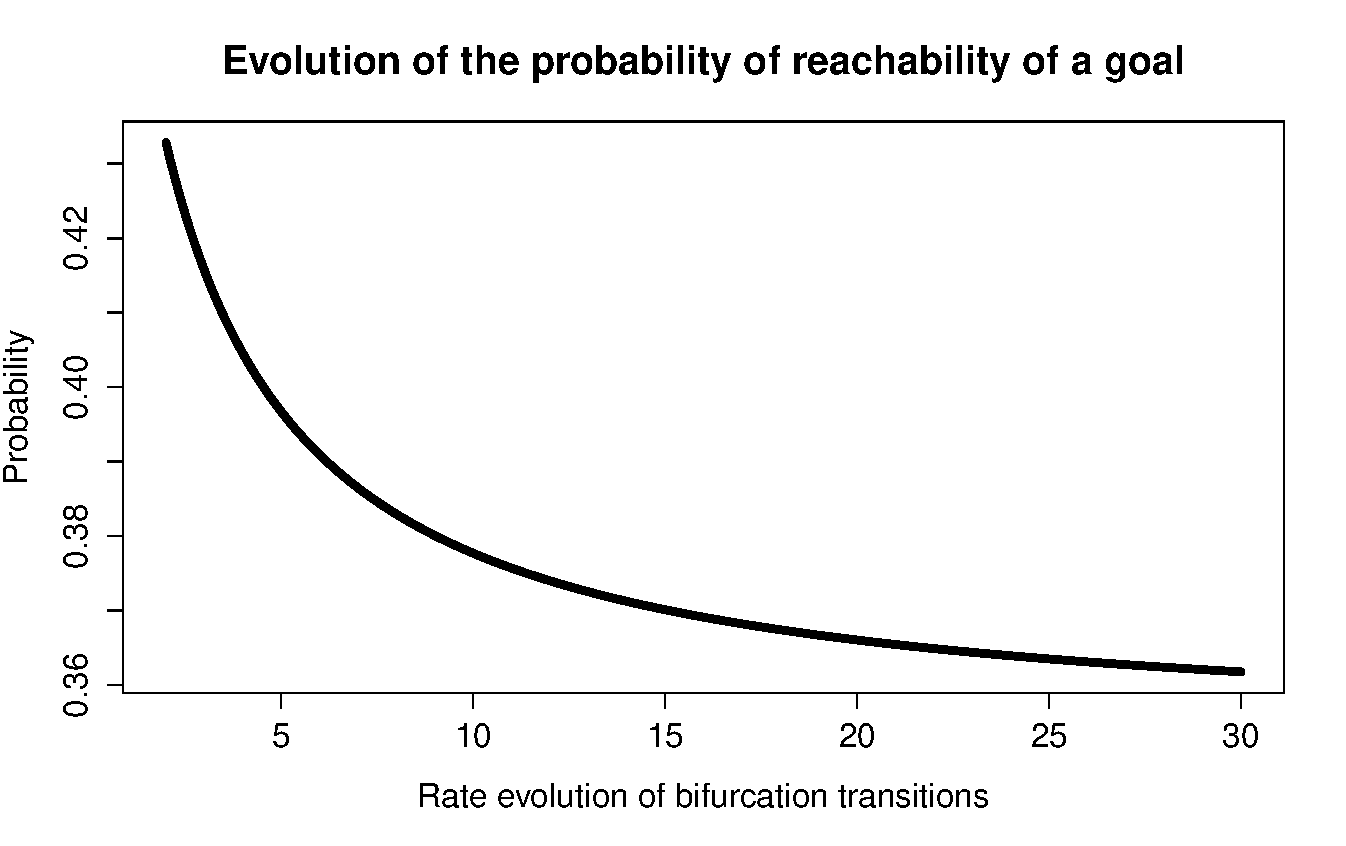
\includegraphics[scale=0.4]{images/prob_evol_new.pdf}
\end{center}
 

\begin{itemize}
 \item PRISM for simulation.
 \item A decrease of the probability of reach $CI=2$ in the lambda phage model from the initial state.
\end{itemize}
 
\end{frame}
\end{comment}
